%
% File acl2018_supp.tex
%

\documentclass[11pt,a4paper]{article}
\usepackage{acl-onecolumn}
\usepackage{times}
\usepackage{url}
\usepackage{latexsym}
\usepackage{amsmath}
\usepackage{breqn}
\usepackage{pgfplotstable}
%\usepackage{algorithm2e}
\usepackage{hhline}
\usepackage{multirow}
\usepackage{multicol}
\usepackage[font=small]{caption}
\usepackage{subcaption}
\usepackage{color}
\usepackage{float}
\usepackage{lipsum,adjustbox}
\usepackage{tikz}
\usepackage{tikz-dependency}
\usepackage{enumitem}
\usepackage{rotating}
\usepackage{xr}
\externaldocument{tupa_multitask}
\usetikzlibrary{shapes,fit,calc,er,positioning,intersections,decorations.shapes,mindmap,trees}
\tikzset{decorate sep/.style 2 args={decorate,decoration={shape backgrounds,shape=circle,
      shape size=#1,shape sep=#2}}}
\newcommand{\oa}[1]{\footnote{\color{red} #1}}
\newcommand{\daniel}[1]{\footnote{\color{blue} #1}}
\newcommand{\com}[1]{}
\DeclareMathOperator*{\argmin}{argmin}
\DeclareMathOperator*{\argmax}{argmax}
%\SetKwRepeat{Do}{do}{while}

\hyphenation{SemEval}
\hyphenation{PARSEVAL}

\title{Multitask Parsing Across Semantic Representations \\ Supplementary Notes}

\begin{document}
\maketitle

\paragraph{Features.}

Table~\ref{tab:features} lists all feature used for the classifier (see \S\ref{sec:classifier}).
Numeric features are taken as they are, whereas categorical features are mapped to real-valued embedding
vectors.
For \texttt{w} features,
we concatenate randomly-initialized and pre-trained word embeddings.
For each node, we select a \textit{head terminal} by traversing the graph according to
a priority order on edge labels, taken from \citet{hershcovich2017a}.

$s_i$ refers to stack node $i$ from the top, and
$b_i$ to buffer node $i$.
$xl$ and $xr$ refer to a $x$'s leftmost and rightmost children, and
$xL$ and $xR$ to its leftmost and rightmost parents.

\texttt{w} refers to the node's head terminal text,
\texttt{t} to its POS tag, and
\texttt{d} to its dependency relation.
\texttt{h} refers to the node's height,
\texttt{e} to the tag of its first incoming edge,
\texttt{n} and \texttt{c} to the node label and category (used only for AMR),
\texttt{p} to any separator punctuation between $s_0$ and $s_1$,
\texttt{q} to the count of any separator punctuation between $s_0$ and $s_1$,
\texttt{x} to the numeric value of gap type \cite{maier-lichte:2016:DiscoNLP},
\texttt{y} to the sum of gap lengths,
\texttt{P}, \texttt{C}, \texttt{I}, \texttt{E}, and \texttt{M} to the number of
parents, children, implicit children, remote children, and remote parents,
\texttt{N} to the numeric value of the head terminal's named entity IOB indicator,
\texttt{T} to its named entity type,
\texttt{\#} to its word shape (capturing orthographic features, e.g. "Xxxx" or "dd"),
\texttt{\^{}} to its one-character prefix, and
\texttt{\$} to its three-character suffix.

$x \to y$ refers to the existing edge from $x$ to $y$.
\texttt{x} is an indicator feature, taking the value of 1 if the edge exists or 0 otherwise,
\texttt{e} refers to the edge label, and
\texttt{d} to the dependency distance between the head terminals of the nodes.

$a_i$ to the transition taken $i+1$ steps ago.
\texttt{A} refers to the action type label (e.g. \textsc{shift}/\textsc{right-edge}/\textsc{node}), and
\texttt{e} to the edge label created by the action (e.g. $C$/$E$/$P$).

\texttt{node ratio} is the ratio between non-terminals and terminals, taken from \citet{hershcovich2017a}.

\begin{table}[h]
\centering
\begin{tabular}{l|l}
\bf Nodes & \bf Features \\ 
\hline
%       w   t   d   e   n   c   p   T   #   ^   $   x   h   q   y   P   C   I   E   M   N
$s_0$ & \texttt{wtdencpT\#\^{}\$xhqyPCIEMN} \\
$s_1$ & \texttt{wtdencT\#\^{}\$xhyN} \\
$s_2$ & \texttt{wtdencT\#\^{}\$xhy} \\
$s_3$ & \texttt{wtdencT\#\^{}\$xhyN} \\
$b_0$ & \texttt{wtdncT\#\^{}\$hPCIEMN} \\
$b_1, b_2, b_3$ & \texttt{wtdncT\#\^{}\$} \\
$s_0l, s_0r, s_1l, s_1r, s_0ll, s_0lr, s_0rl, s_0rr, s_1ll, s_1lr, s_1rl, s_1rr$ &
    \texttt{wenc\#\^{}\$} \\
$s_0L, s_0R, s_1L, s_1R, b_0L, b_0R$ & \texttt{wen\#\^{}\$} \\
\hline
\bf Edges & \\
$s_0 \to s_1, s_0 \to b_0$ & \texttt{xd} \\
$s_1 \to s_0, b_0 \to s_0$ & \texttt{x} \\
$s_0 \to b_0, b_0 \to s_0$ & \texttt{e} \\
\hline
\bf Past actions \\
$a_0, a_1$ & \texttt{eA} \\
\hline
\bf Misc. & \texttt{node ratio}
\end{tabular}
\caption{Transition classifier features.\label{tab:features}}
\end{table}


\paragraph{Conversion to and from Unified DAG Format.}

Although all experiments reported in the paper with the auxiliary tasks
(AMR, DM and UD) are using unlabeled parsing for these schemes,
our conversion code supports full conversion to and from these formats,
and is publicly available at \url{http://github.com/danielhers/semstr/tree/master/semstr/conversion}.

Conversion from AMR to the unifid DAG format and back
results in 95\% Smatch $F_1$ \cite{cai2013smatch} when averaged over the
LDC2017T10 test set.
On SDP, the conversion is lossless and results in identical graphs
when converted to UCCA and back.
For UD, and conversion results in 98.5\% LAS $F_1$ on the UD English test set,
due to multi-word tokens, not supported in the unified DAG format.

\paragraph{Qualitative evaluation.}

Figure~\ref{fig:qualitative} shows an example sentence from the English 20K test set,
with the outputs of both our single-task model and our best MTL model (using all auxiliaries).
While the single-task model obtains an $F_1$ score of 67.9\% on this sentence, the MTL model's output
matches the gold-annotates graph perfectly.
This example demonstrates how
the parser's ability to identify syntactic constituents,
which is important for all tasks we tackled, is improved with MTL.


\begin{sidewaysfigure}
    \centering
\scalebox{.6}{
\begin{tikzpicture}[->,level distance=26mm,
  level 1/.style={sibling distance=16cm},
  level 2/.style={sibling distance=7cm},
  level 3/.style={sibling distance=2cm},
  every circle node/.append style={fill=black}]
  \tikzstyle{word} = [font=\rmfamily,color=black]
  \node (1_1) [circle] {}
  {
  child {node (1_2) [circle] {}
    {
    child {node (1_5) [circle] {}
      {
      child {node (1_10) [word] {No} edge from parent node[auto] {\scriptsize $E$}}
      child {node (1_11) [word] {transoceanic} edge from parent node[auto] {\scriptsize $E$}}
      child {node (1_12) [word] {navigational} edge from parent node[auto] {\scriptsize $E$}}
      child {node (1_13) [word] {undertaking} edge from parent node[auto] {\scriptsize $C$}} }edge from parent node[auto] {\scriptsize $A$}}
    child {node (1_6) [circle] {}
      {
      child {node (1_14) [word] {has} edge from parent node[auto] {\scriptsize $F$}}
      child {node (1_15) [word] {been} edge from parent node[auto] {\scriptsize $E$}}
      child {node (1_16) [word] {conducted} edge from parent node[auto] {\scriptsize $C$}} }edge from parent node[auto] {\scriptsize $P$}}
    child {node (1_7) [circle] {}
      {
      child {node (1_17) [word] {with} edge from parent node[auto] {\scriptsize $R$}}
      child {node (1_18) [circle] {}
        {
        child {node (1_25) [circle] {}
          {
          child {node (1_28) [word] {more} edge from parent node[auto] {\scriptsize $E$}}
          child {node (1_29) [word] {ability} edge from parent node[auto] {\scriptsize $C$}} }edge from parent node[auto] {\scriptsize $C$}}
        child {node (1_26) [word] {,} edge from parent node[auto] {\scriptsize $U$}}
        child {node (1_27) [circle] {}
          {
          child {node (1_30) [word] {no} edge from parent node[auto] {\scriptsize $E$}}
          child {node (1_31) [circle] {}
            {
            child {node (1_32) [word] {business} edge from parent node[auto] {\scriptsize $E$}}
            child {node (1_33) [word] {dealings} edge from parent node[auto] {\scriptsize $C$}} }edge from parent node[auto] {\scriptsize $C$}} }edge from parent node[auto] {\scriptsize $C$}} }edge from parent node[auto] {\scriptsize $C$}} }edge from parent node[auto] {\scriptsize $A$}} }edge from parent node[auto] {\scriptsize $H$}}
  child {node (1_3) [circle] {}
    {
    child {node (1_8) [circle] {}
      {
      child {node (1_19) [word] {have} edge from parent node[auto] {\scriptsize $F$}}
      child {node (1_20) [word] {been} edge from parent node[auto] {\scriptsize $E$}}
      child {node (1_21) [word] {crowned} edge from parent node[auto] {\scriptsize $C$}} }edge from parent node[auto] {\scriptsize $P$}}
    child {node (1_9) [circle] {}
      {
      child {node (1_22) [word] {with} edge from parent node[auto] {\scriptsize $R$}}
      child {node (1_23) [word] {greater} edge from parent node[auto] {\scriptsize $D$}}
      child {node (1_24) [word] {success} edge from parent node[auto] {\scriptsize $P$}} }edge from parent node[auto] {\scriptsize $A$}} }edge from parent node[auto] {\scriptsize $H$}}
  child {node (1_4) [word] {.} edge from parent node[auto] {\scriptsize $U$}} }
;
\end{tikzpicture}}
\scalebox{.6}{
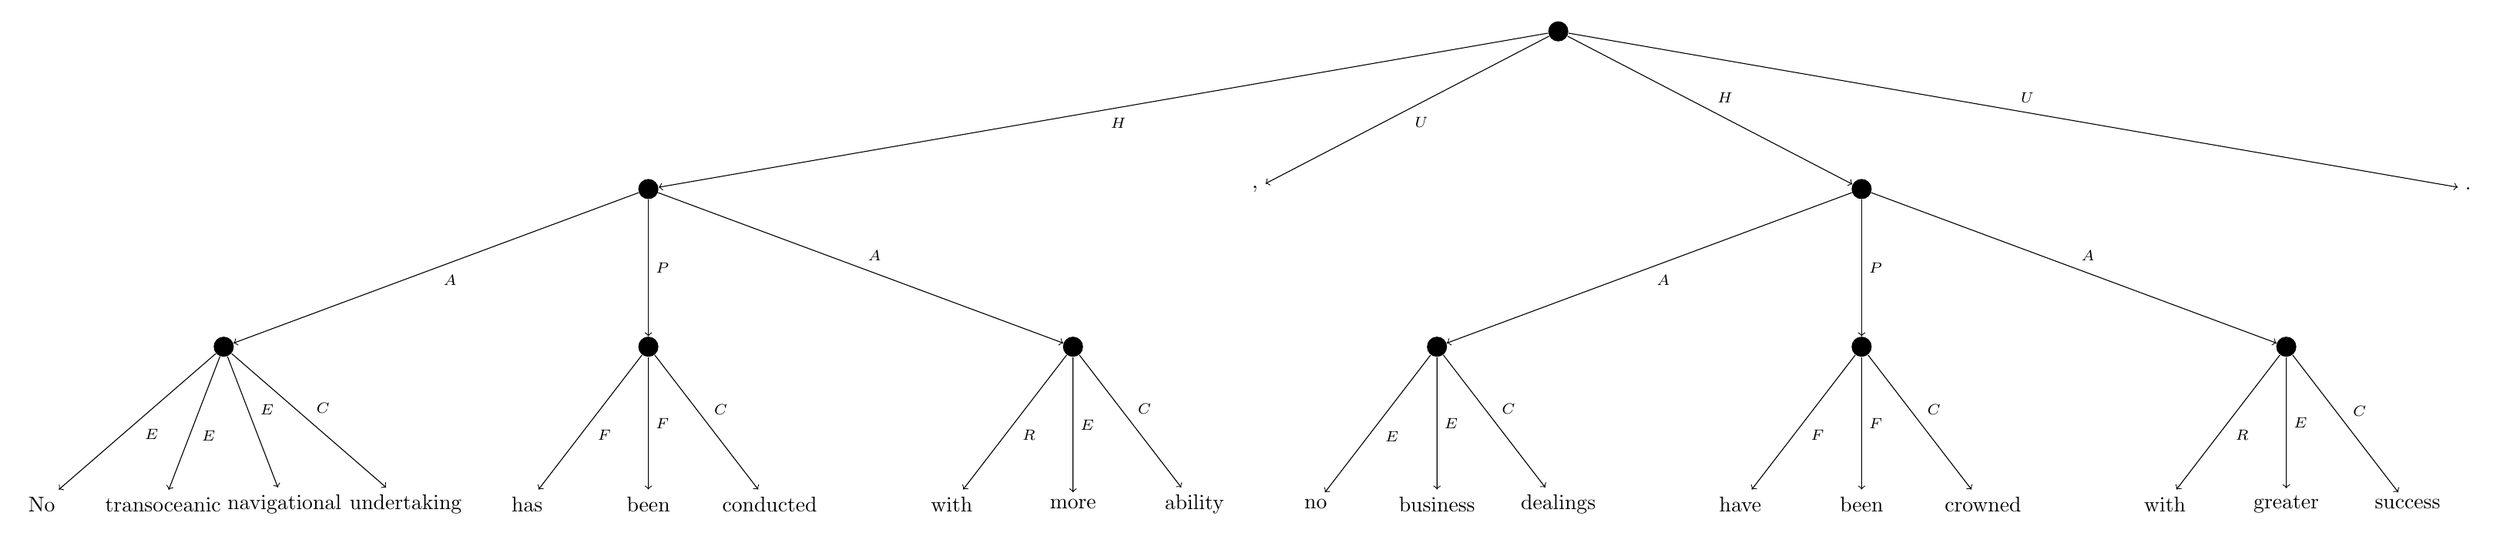
\begin{tikzpicture}[->,level distance=26mm,
      level 1/.style={sibling distance=10cm},
      level 2/.style={sibling distance=7cm},
      level 3/.style={sibling distance=2cm},
  every circle node/.append style={fill=black}]
  \tikzstyle{word} = [font=\rmfamily,color=black]
  \node (1_1) [circle] {}
  {
  child {node (1_2) [circle] {}
    {
    child {node (1_6) [circle] {}
      {
      child {node (1_12) [word] {No} edge from parent node[auto] {\scriptsize $E$}}
      child {node (1_13) [word] {transoceanic} edge from parent node[auto] {\scriptsize $E$}}
      child {node (1_14) [word] {navigational} edge from parent node[auto] {\scriptsize $E$}}
      child {node (1_15) [word] {undertaking} edge from parent node[auto] {\scriptsize $C$}} }edge from parent node[auto] {\scriptsize $A$}}
    child {node (1_7) [circle] {}
      {
      child {node (1_16) [word] {has} edge from parent node[auto] {\scriptsize $F$}}
      child {node (1_17) [word] {been} edge from parent node[auto] {\scriptsize $F$}}
      child {node (1_18) [word] {conducted} edge from parent node[auto] {\scriptsize $C$}} }edge from parent node[auto] {\scriptsize $P$}}
    child {node (1_8) [circle] {}
      {
      child {node (1_19) [word] {with} edge from parent node[auto] {\scriptsize $R$}}
      child {node (1_20) [word] {more} edge from parent node[auto] {\scriptsize $E$}}
      child {node (1_21) [word] {ability} edge from parent node[auto] {\scriptsize $C$}} }edge from parent node[auto] {\scriptsize $A$}} }edge from parent node[auto] {\scriptsize $H$}}
  child {node (1_3) [word] {,} edge from parent node[auto] {\scriptsize $U$}}
  child {node (1_4) [circle] {}
    {
    child {node (1_9) [circle] {}
      {
      child {node (1_22) [word] {no} edge from parent node[auto] {\scriptsize $E$}}
      child {node (1_23) [word] {business} edge from parent node[auto] {\scriptsize $E$}}
      child {node (1_24) [word] {dealings} edge from parent node[auto] {\scriptsize $C$}} }edge from parent node[auto] {\scriptsize $A$}}
    child {node (1_10) [circle] {}
      {
      child {node (1_25) [word] {have} edge from parent node[auto] {\scriptsize $F$}}
      child {node (1_26) [word] {been} edge from parent node[auto] {\scriptsize $F$}}
      child {node (1_27) [word] {crowned} edge from parent node[auto] {\scriptsize $C$}} }edge from parent node[auto] {\scriptsize $P$}}
    child {node (1_11) [circle] {}
      {
      child {node (1_28) [word] {with} edge from parent node[auto] {\scriptsize $R$}}
      child {node (1_29) [word] {greater} edge from parent node[auto] {\scriptsize $E$}}
      child {node (1_30) [word] {success} edge from parent node[auto] {\scriptsize $C$}} }edge from parent node[auto] {\scriptsize $A$}} }edge from parent node[auto] {\scriptsize $H$}}
  child {node (1_5) [word] {.} edge from parent node[auto] {\scriptsize $U$}} }
;
\end{tikzpicture}}
\caption{Output of single-task model on sentence 53001 from the English 20K test set (top),
and of MTL model using all of AMR, DM and UD$^{++}$ as auxiliaries on the same sentence (bottom).
\label{fig:qualitative}}
\end{sidewaysfigure}

\bibliography{references}
\bibliographystyle{acl_natbib}

\end{document}
